\documentclass[a4paper, notitlepage, oneside]{article}

\usepackage[english]{babel}
\usepackage[latin1]{inputenc}
\usepackage[T1]{fontenc}

\usepackage{graphicx}
\usepackage{hyperref}

\DeclareGraphicsExtensions{.png,.jpg}

\begin{document}
\title{MassIdea User Experience Study}
\author{Jan Michael Auer \and Tobias Curth}
\date{Hagenberg, April 2012}
\maketitle

\vspace{3cm}

\begin{abstract}
This paper contains a study targeting a whole new user experience in the next version of MassIdea.org along with some early drafts for a fresh and modern user interface. The main focus lies on the overall experience a user should have browsing MassIdea.org.
\end{abstract}
\pagebreak

\tableofcontents
\pagebreak

\section{Wireframe}
\label{sec:wireframe}

The basic wireframe describes a general structure of every page hosted on massidea.org. It is divided into three sections.

\begin{figure}[htb]
	\centering
	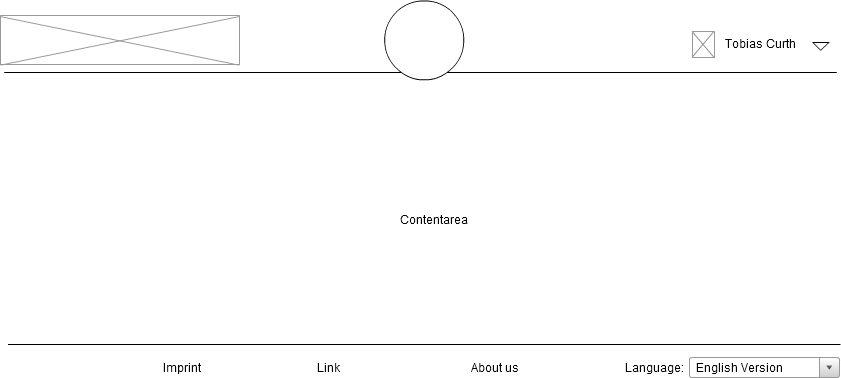
\includegraphics[width=0.95\textwidth]{wire}
	\caption{The basic wireframe of MassIdea 2.0 showing header, content and footer}
	\label{fig:wireframe}
\end{figure}

\begin{description}
	\item[Header] \hfill \\
	The header is almost identical on every page the user visits. The most catchy object is the \emph{MassIdea logo} in the middle, which is slightly breaking with the header frame. On the left there is the \emph{MassIdea lettering} along with a the slogan, which always links to the home page. On the right there is either a login form along with a link for signing up or a user menu to access the own profile, preferences and log out. 
	\item[Content] \hfill \\
	This part of the page always adapts to the context of the page. It may contain a sidebar, pictures and text, as well as animations.
	\item[Footer] \hfill \\
	The most narrow part of the page is at the bottom, containing links to the imprint and the about page, a copyright disclaimer and a language selector which changes the language of all user interface elements.
\end{description}

The \emph{language selector} field in the very bottom of the page thereby plays an essential role, since users are able to adjust the language of all elements on the page and not only contents. Storing this preference in cookies or in user account settings - if logged in - is  advisable.

Another important element is the \emph{user menu} seen in figure~\ref{fig:wireframe} in the top right corner. It provides the user with a convenient way to access important pages by navigating through a neatly arranged menu.

In general, the page adapts a modern and lightweight \emph{Web 2.0} style, leaving enough space for the user to feel well and having all necessary but not too many user interface elements on the screen. Anyway, the design is rather timeless than ultra modern to be appropriate in future too.

\section{Public Start Page}
\label{sec:public}

The public start page is only shown to users who are not logged in. Therefore, its main task is to inform about MassIdea, challenges, ideas and visions. Thus, it utilizes the \emph{AIDA principle}.

\subsection{The AIDA Principle}

The AIDA principle, originally an acronym used in marketing and advertising, is one of the most important guidelines for user interface desigers. It is used to attract potential users and create some sort of temption to buy or join.

\begin{description}
	\item[Attention] Attract the user's attention with a catchy image or an animation.
	\item[Interest] Raise interest by focusing on advantages and benefits.
	\item[Desire] Create a demand for the advertised product and declare that the product will satisfy all needs
	\item[Action] Lead customers towards taking action - as simple as possible
\end{description}

For further information visit \url{http://en.wikipedia.org/wiki/AIDA_(marketing)}.

\subsection{Start Page Layout}

\begin{figure}[htb]
	\centering
	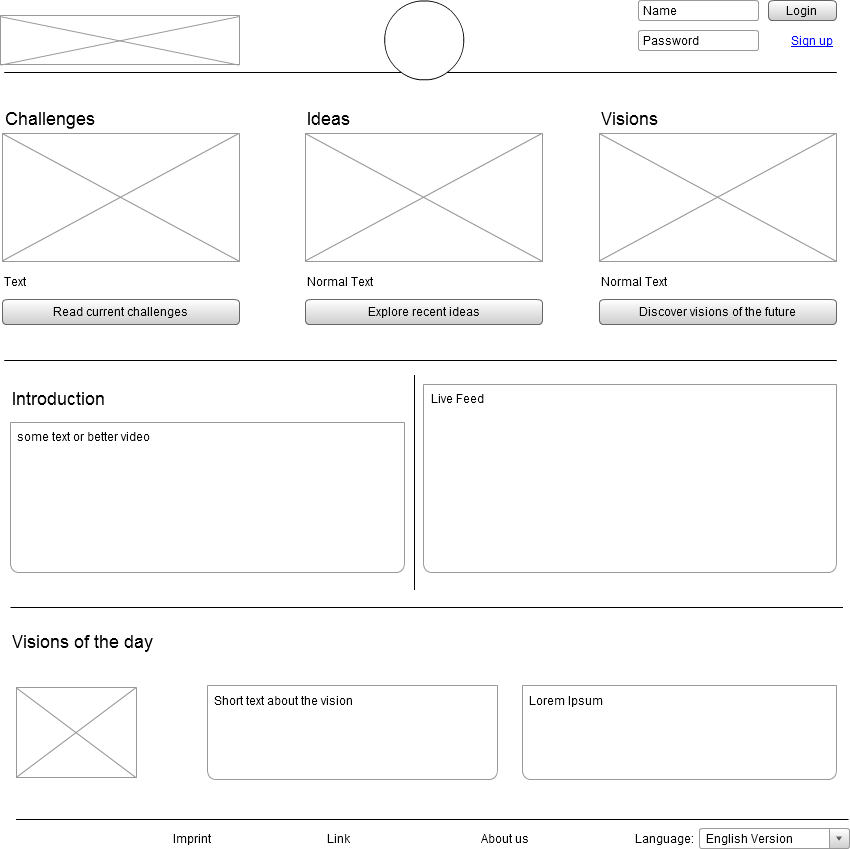
\includegraphics[width=0.95\textwidth]{home}
	\caption{The public start page utilizing the AIDA principle.}
	\label{fig:home}
\end{figure}

In order to get startet quickly and learn as much as possible about challenges, ideas and visions in short time, there is a brief introduction on the start page right away. Catchy images and short texts help to identify the sections easily. The images used on the start page are also used for all posts in these sections for better recognition. The texts consist of a short (about 2 - 3 lines) description of meaning and differences. 

Below, buttons refer to landing pages, where public feeds of challenges, ideas and visions are presented to the user (see section~\ref{sec:feeds}). Clicking anywhere else on these elements brings up a \emph{popover dialog} to write a new post immediately (see section~\ref{sub:public_post}).

Underneath, there's an introduction describing what the intention behind MassIdea is and how to get started. This introduction can also be a short video or animation (e.g. \url{http://www.apple.com/ipad}). It contains information about what MassIdea is, how to use it and an invitation to sign up.

Next to the introduction a pseudo-live feed shows some random articles popping up every few sections. This does not only raise attention but also trigger the user's interest.

At the very bottom a featured "post of the day" (e.g. a vision) is presented. These featured posts are successful case studies, chosen out of a pool of preselected completed challenges. The intention behind this is to show the success of MassIdea and create the desire to participate.

\subsection{Creating a New Post}
\label{sub:public_post}

\begin{figure}[htb]
	\centering
	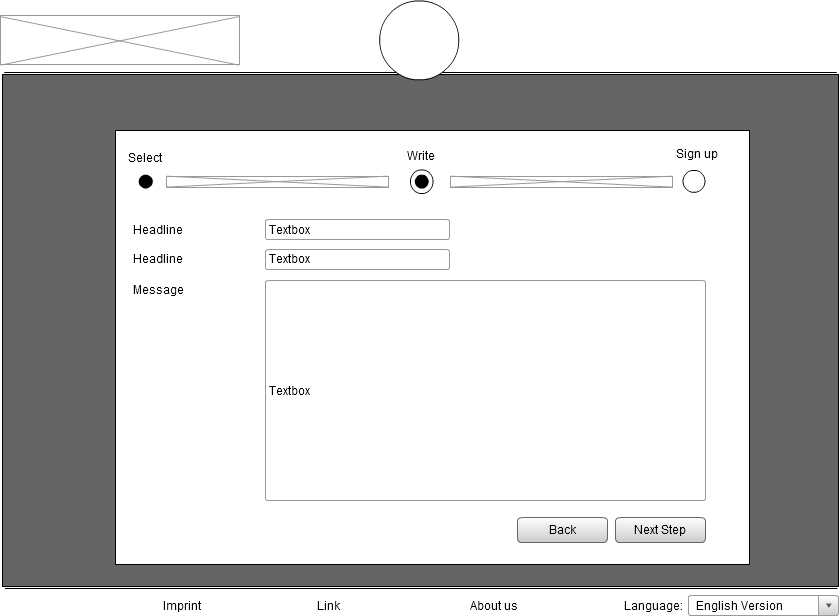
\includegraphics[width=0.95\textwidth]{post}
	\caption{Writing a new post and signig up made simple.}
	\label{fig:post}
\end{figure}

Since users join to create a new post, this process must be easy, fast and intuitive. Therefore it is divided into three steps:

\begin{enumerate}
	\item Selecting the \emph{post type} (challenge, idea or vision)
	\item Writing the post and attaching all documents
	\item Signing up quickly
\end{enumerate}

The order is essential. When users have already written their whole post body and attached all documents when they are prompted to register, they will more likely perform this step. 

That, however, implies that signing up does not require too much personal information. An optimal compromise is to only require name, email and password. Everything else can also be configured later in the profile screen.

During this process, users are always informed about their progress by a three-step progress bar at the top. Beneath, they can compose their post and proceed submitting. Once the user has signed up successfully, the written post is visible and online immediately.

\section{Feeds}
\label{sec:feeds}

As soon as users log in, they are redirected to their personal feed. This feed contains a mixture of recent posts in his favorite groups and sometimes also randomly chosen content. Almost every other page they can access now is also a feed - therefore feeds are a \emph{central hub in MassIdea}. Once users get used to the feeds - and they already have thanks to \emph{Facebook} - they are presented with a clean and consistent user interface wherever they go.

Feeds usually contain challenges, ideas and visions, but they can also host more content to support colaborative work or educational approaches. For more information about special feeds, head over to section~\ref{sec:special_feed}.

\subsection{Generic Feed Layout}
The generic feed layout is knowingly very similar to \emph{social networks} like \emph{Yammer} or \emph{Facebook} due to the fact that millions of users use them every day and are accustomized to their user interfaces, which are indeed very similar.

\begin{description}
	\item[Search Bar] In the side bar, every feed can be searched for several keywords. Search results are presented as soon as the user starts typing, containing and grouped by \emph{users}, \emph{categories} and \emph{posts}.
	\item[Menu Bar] Equally aside, a menu bar enables the user to browse the different feeds and categories. These menu entries redirect the user to a filtered feed, containing only posts matching the actual context.
	\item[Favorites] Especially very active users also attend many groups and follow even more category feeds. To help with that, they can define favorites for quick access over the menu bar. 
	\item[Write New Post] Above every feed, a separate bar enables the user to write new posts (in standard feeds that is, again: challenges, ideas and visions). 
	\item[Feed] The feed itself contains heading, author, excerpt and a \emph{read more} link. For quick interaction, users can also rate the post as well as jump to all linked posts directly from the feed. Each post is colored according to the post type and labeled with an image for immediate recognition. 
	\item[Context Menu] The lambs ear in the top right corner triggers a context menu for further actions, like controlling visibility or attaching a new document.
\end{description}

\begin{figure}[htb]
	\centering
	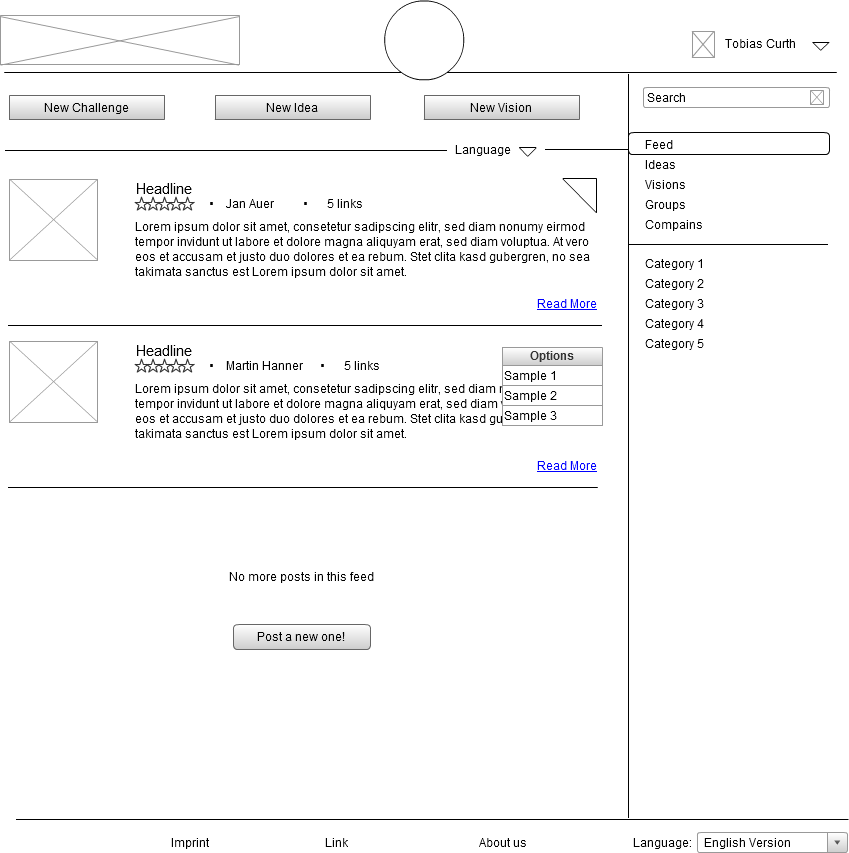
\includegraphics[width=0.95\textwidth]{feed}
	\caption{The feed - a central hub in MassIdea.}
	\label{fig:feed}
\end{figure}

Similar to tools like \emph{Flowdock}, the feed automatically updates with new posts or messages so the user does not have to refresh the page manually every few minutes. 

\subsection{Creating a New Post}

To create a new post, users only have to click on the button naming the right post type and can start to edit right away. This could be done in a \emph{popover dialog} like on the start page, or directly in the feed.

\subsection{Special Feeds}
\label{sec:special_feed}

Besides having the right idea and being able to share it with the whole world, it is also important to find the right people to work with and transform a vision into reality - something that is possible , but rather not intuitive in \emph{MassIdea} right now. 

Special feeds, however, focus on that point and support colaborative work and educational approaches on a very basic level. A good example for such a special feed is a \emph{Group}, where all members work on the same context. Those feeds provide an additional facility to share \emph{Documents} and \emph{Announcements} separately, as they are linked clearly to the group's context. 

\begin{figure}[htb]
	\centering
	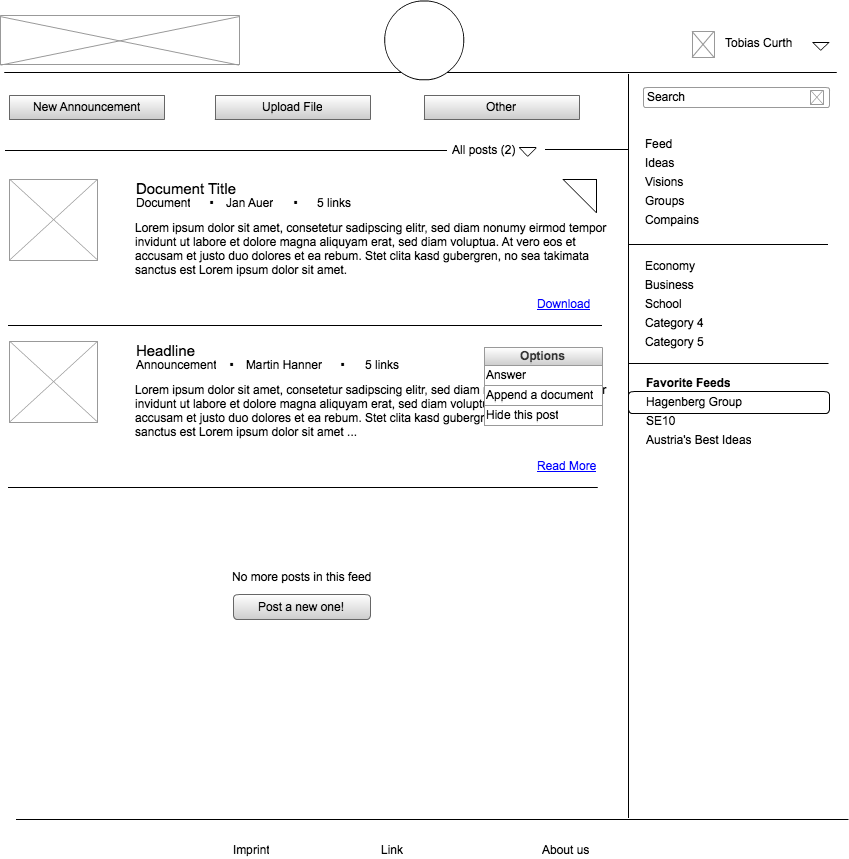
\includegraphics[width=0.95\textwidth]{special}
	\caption{Special feeds enhance the social experience and educational capabilities.}
	\label{fig:special}
\end{figure}
\pagebreak
Users can discuss those documents and announcements or even attach further documents as an "answer". The language filter of standard feeds is replaced by a filter for certain \emph{post types}. Users so can look at documents or announcements exclusively. 

Additionally, the author of such postings is able to specify the visibility of all answers. For example, a teacher uploads the homework assignment for his class and sets answer visibility to false. Students can now upload their results by answering to this post but cannot see other uploaded documents.

\end{document}